% THIS IS SIGPROC-SP.TEX - VERSION 3.1
% WORKS WITH V3.2SP OF ACM_PROC_ARTICLE-SP.CLS
% APRIL 2009
%
% It is an example file showing how to use the 'acm_proc_article-sp.cls' V3.2SP
% LaTeX2e document class file for Conference Proceedings submissions.
% ----------------------------------------------------------------------------------------------------------------
% This .tex file (and associated .cls V3.2SP) *DOES NOT* produce:
%       1) The Permission Statement
%       2) The Conference (location) Info information
%       3) The Copyright Line with ACM data
%       4) Page numbering
% ---------------------------------------------------------------------------------------------------------------
% It is an example which *does* use the .bib file (from which the .bbl file
% is produced).
% REMEMBER HOWEVER: After having produced the .bbl file,
% and prior to final submission,
% you need to 'insert'  your .bbl file into your source .tex file so as to provide
% ONE 'self-contained' source file.
%
% Questions regarding SIGS should be sent to
% Adrienne Griscti ---> griscti@acm.org
%
% Questions/suggestions regarding the guidelines, .tex and .cls files, etc. to
% Gerald Murray ---> murray@hq.acm.org
%
% For tracking purposes - this is V3.1SP - APRIL 2009

\documentclass{acm_proc_article-sp}


\usepackage{url}
\usepackage{graphicx}

\usepackage{bera}% optional: just to have a nice mono-spaced font
\usepackage{listings}
\usepackage{xcolor}

\colorlet{punct}{red!60!black}
\definecolor{background}{HTML}{EEEEEE}
\definecolor{delim}{RGB}{20,105,176}
\colorlet{numb}{magenta!60!black}

\lstdefinelanguage{json}{
    basicstyle=\normalfont\ttfamily,
    numbers=left,
    numberstyle=\scriptsize,
    stepnumber=1,
    numbersep=8pt,
    showstringspaces=false,
    breaklines=true,
    frame=lines,
    backgroundcolor=\color{background},
    literate=
     *{0}{{{\color{numb}0}}}{1}
      {1}{{{\color{numb}1}}}{1}
      {2}{{{\color{numb}2}}}{1}
      {3}{{{\color{numb}3}}}{1}
      {4}{{{\color{numb}4}}}{1}
      {5}{{{\color{numb}5}}}{1}
      {6}{{{\color{numb}6}}}{1}
      {7}{{{\color{numb}7}}}{1}
      {8}{{{\color{numb}8}}}{1}
      {9}{{{\color{numb}9}}}{1}
      {:}{{{\color{punct}{:}}}}{1}
      {,}{{{\color{punct}{,}}}}{1}
      {\{}{{{\color{delim}{\{}}}}{1}
      {\}}{{{\color{delim}{\}}}}}{1}
      {[}{{{\color{delim}{[}}}}{1}
      {]}{{{\color{delim}{]}}}}{1},
}


\begin{document}

\title{IN4392 Cloud Computing}
\subtitle{CloudSearch Report}
%
% You need the command \numberofauthors to handle the 'placement
% and alignment' of the authors beneath the title.
%
% For aesthetic reasons, we recommend 'three authors at a time'
% i.e. three 'name/affiliation blocks' be placed beneath the title.
%
% NOTE: You are NOT restricted in how many 'rows' of
% "name/affiliations" may appear. We just ask that you restrict
% the number of 'columns' to three.
%
% Because of the available 'opening page real-estate'
% we ask you to refrain from putting more than six authors
% (two rows with three columns) beneath the article title.
% More than six makes the first-page appear very cluttered indeed.
%
% Use the \alignauthor commands to handle the names
% and affiliations for an 'aesthetic maximum' of six authors.
% Add names, affiliations, addresses for
% the seventh etc. author(s) as the argument for the
% \additionalauthors command.
% These 'additional authors' will be output/set for you
% without further effort on your part as the last section in
% the body of your article BEFORE References or any Appendices.

\numberofauthors{5} %  in this sample file, there are a *total*
% of EIGHT authors. SIX appear on the 'first-page' (for formatting
% reasons) and the remaining two appear in the \additionalauthors section.
%
\author{
% You can go ahead and credit any number of authors here,
% e.g. one 'row of three' or two rows (consisting of one row of three
% and a second row of one, two or three).
%
% The command \alignauthor (no curly braces needed) should
% precede each author name, affiliation/snail-mail address and
% e-mail address. Additionally, tag each line of
% affiliation/address with \affaddr, and tag the
% e-mail address with \email.
%
% 1st. author
\alignauthor
R. Cioromela\\
	\affaddr{Author}\\
    \email{r.cioromela@}
% 2nd. author
\alignauthor
V. Ghiette\\
	\affaddr{Author}\\
    \email{v.d.h.ghiette@\{student.tudelft.nl\}}
% 3rd. author
\and 
\alignauthor 
A. Iosup\\
	\affaddr{Course instructor}\\
	\affaddr{PDS Group, EEMCS, TU Delft}\\
      	 \email{A.Iosup@tudelft.nl}
 % use '\and' if you need 'another row' of author names
% 4th. author
\alignauthor 
D. Epema\\
	\affaddr{Course instructor}\\
	\affaddr{PDS Group, EEMCS, TU Delft}\\
      	 \email{D.H.J.Epema@tudelft.nl}
% 5th. author
\alignauthor
B. Ghit\\
	\affaddr{Lab assistant}\\
	\affaddr{PDS Group, EEMCS, TU Delft}\\
      	 \email{B.I.Ghit@tudelft.nl}
}
\maketitle

\begin{abstract}
In this report, we introduce a cloud application that provides search functionality through news articles.
The application is called CloudSearch and uses natural language processing to provide search results.
The application is a showcase which can be used to illustrate the advantages of cloud computing in company settings.
In the report the development and the deployment of the application are presented and test results are discussed.
\end{abstract}

\section{Introduction}
This report focuses on the use of Internet as a Service (IaaS) to help companies provide their services to users.
In this report the development, implementation, deployment, and performance analysis of a service deployed on a cloud platform is illustrated.
In order to illustrate this, a new developped service CloudSearch is used.
CloudSeach (CS) is a search engine which offers the users the possibility to search for relevant news articles.\\
First a brief overview of the CS application is given.
Then an elaborate system design is presented to illustrate the deployment of the CS application on a cloud platform.
Finally test results are provided followed by a conclusion.

\section{CloudSearch}
The CloudSearch application is a search engine, the application returns relevant news articles given the user's search input.
The application can be split into three parts, the front end, and the back end which consist of master and slave nodes, shown in Figure \ref{fig:overview}.
\begin{figure}[ht!]
\centering
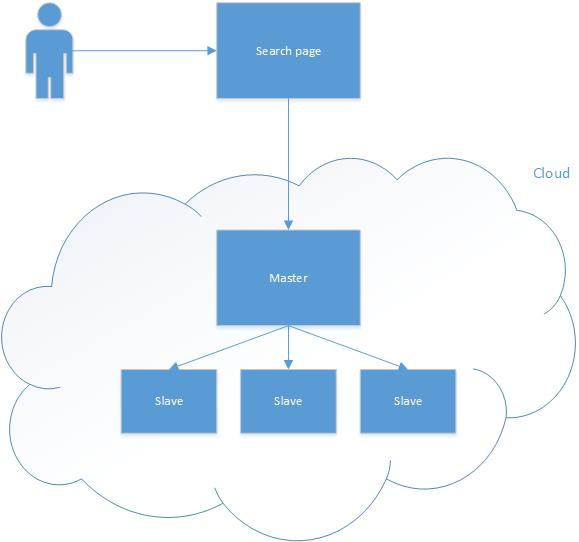
\includegraphics[scale=0.5]{CloudSearchOverview.jpg}
\caption{CloudSearch overview \label{fig:overview}}
\end{figure}
The front end is a web page which takes the user input and sends it to the master node.
The input are person, location, and organisation names.
These names are sent to the master node.\\
The master node  splits the query into sub queries which are sent to the available slave nodes.
This is done by assigning each slave a subset of all the news articles.\\
The slave then parses the given subset of articles and extracts all the person, location and organisation names from the text.
Then these names are compared to the query and the relevant texts are sent back to the master.\\
The master merges the results from the slaves and sends the final response back to the front end.\\
The front end displays the results on the web page, the results show all the names in the texts and their occurrences in the texts.
This allows the users to establish links between names based on their occurrence in the same text.
For instance if a user searcher for \textit{Bill} the results may indicate that there is a relation between \textit{Bill} and \textit{The white house}.\\

The master and slave nodes must be located in the cloud, however the front end does not.
The front end may be hosted by the user itself.
This is possible because the front end only uses JavaScript to send the queries to the master nodes.
For accessibility the front end may also be hosted in the cloud or even on a git-hub as the only dependency the front end has, besides the need for an internet connection, is the need for a web-browser.\\
More information concerning the cloud search application can be found in Appendix \ref{app:detCS}.

\section{System Design}
The system design is based on using the Amazon cloud service (AWS).
In Figure \ref{fig:detailed} a detailed overview is given from the different components used to make CloudSearch run in a cloud environment.

\begin{figure}[ht!]
\centering
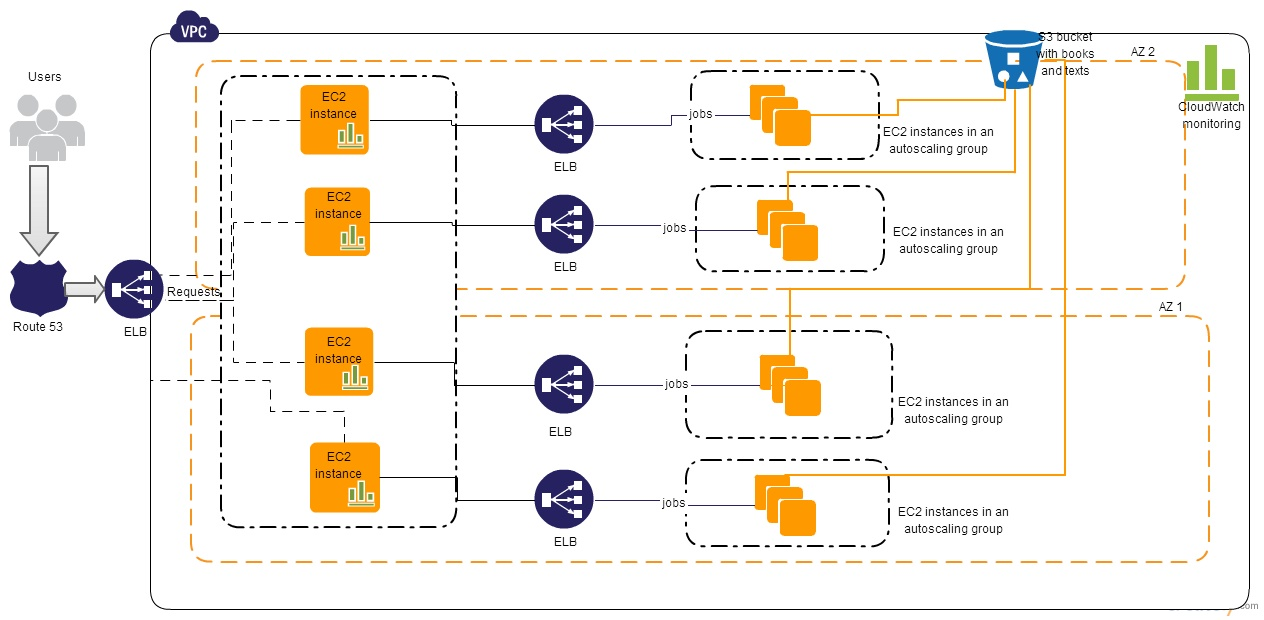
\includegraphics[scale=0.5, angle=90]{CloudSearchDetailed.jpg}
\caption{CloudSearch system design \label{fig:detailed}}
\end{figure}

In more details, a Virtual Private Cloud (VPC) is created in AWS, where the whole  infrastucture resides.
The VPC contains a public subnet and a private subnet. 
In the public subnet there is the webclient, the bastion, and the elastic load balancer for the Splitters machine.
The splitter machines are the master nodes and have the role to receive the query requests and split the request further in smaller requests. 
In the private subnet there are the Splitters (the EC2 instances that receive the requests from the webclient via the SplitterLoadBalancer), the WorkerLoadBalancer that will receive the smaller requests from the Splitters, the Workers (the actual end point that will solve the task). 
The Bastion has the role to administrate the infrastructure and represents an access point to all the machines, in case of manual intervention need.
The Splitters and the Workers are also in auto scaling groups, so when their CPU usage exceeds a certain percentage, a scaling policy is triggered and that will trigger the creation of new machines, until the load can be easily handled. 
The machines are created uniformly in two availability zones, so that the system can be highly available - in case one of the availability zones of region Frankfurt disappears, the other availability zone can take over and create there more workers and splitters. 
The only points of failures would be the webclient and the bastion. 
But because the bastion doesn't have a significant role in the architecture, it can be later replaced. 
For the Webclient, an alarm will be triggered and an email will be sent to the administrators, that will take care of it and recreate the machine. 
However, the probability that an AWS AZ will completely dissapear is very unlikely to happen.

In our tests we used small machines, the free tiers from AWS, to reduce costs. 
The performance of the program can be significantly increased when using more performant EC2 instances. 


\subsection{Used Services}
In order to implement the CloudSearch into the cloud several services offered by AWS are used.
First Virtual Privatye Cloud (VPC) is used. 
As the name states VPC is used to create a private cloud, that is to assure full controle over the cloud environment.
Furthermore, Cloudformation is used to reduce the deployment time. 
It facilitates the automatic deployment of the whole infrastructure, by providing a json file with the description of the resources wanted and embedded scripts that will bootstrap the resources.
Also, CloudWatch is used to monitor the cloud environment, it allows for the creation of monitoring conditions and alarm creation.
S3 is a storage service provided by AWS and handles the data storage, which is the storage of news articles.
Finally EC2 instances are used to run the software. 
EC2 are virtual machines which run in the VPC, these instance can vary in performance, that is EC2 instance can be chosen to be powerful or mediocre machine.
During the entire deployment micro type instance are used due to their costs.\\
In order to ensure good response times the chosen AWS region to run CS is Frankfurt as it is the closest AWS location.

\subsection{Security measures}
The architecture has a three layer security, at the physical, network, and group level.\\
The physical environment, which is secured by AWS. 
All the datacenters of AWS are highly secured and nobody can reach them without special authorization.\\
At the network level, when using a virtual private cloud in AWS, it is possible to build your own virtual network infrastructure. \\
Therefore, it is possible to use Access Control Lists, that allow IP white listing.\\
The security group - the security group is the closest level to the virtual instance. 
At this level, ports can be open to the whitelisted IPs or other security groups, when interaction between different type of components is needed.\\
Another important security measure is not uploading direct code to AWS (S3 or instances), but jars. 
We wouldn't like third parties to have access to our code, so we don't store any direct java code in AWS. 
The only files that will be stored in AWS are the deployment files, in the future it can be improved and configure AWS to deploy from a Git repository, however in order to achieve this, a Beanstalk service is needed.

\subsection{Monitoring}
Monitoring is performed by Cloudwatch. 
Cloudwatch is a tool provided by AWS, where the users can define their own metrics or use pre-defined ones and receive alerts on them. 
Cloudwatch has pre-defined metrics that monitors the CPU or memory usage of the machines, network and a series of other characteristics, specific to each type of hardware used. 
The system behind Cloudwatch checks the monitored resources every 5 minutes by default (the free monitoring) or every 1 minute (when the users need to pay an extra fee). 
The users can also post to Cloudwatch their own metrics and get alerts on it, when certain thresholds are reached or exceeded. 
An example of the used monotor settings is available in Appendix \ref{app:exCA}.

\subsection{Scaling}
For scaling the CPU usage of the created EC2 instance is monitored.
Only CPU based scaling is used as no apparent time pattern of the application's usage can be determined.
One important feature from AWS that is used in the scaling design is the auto scaling group. 
It acts like a fence around the group of EC2 instances, and it can create or terminate automatically the EC2 instances, according to the needs. 
It is in a close relation with the Cloudwatch alarms and the scaling policies. 
When a Cloudwatch alarm is triggered, the scaling policies act accordingly and new machines are added or removed from the autoscaling group. 
In the autoscaling group, we could set also the maximum number of machines that we can scale to.  
For instance, during research, we wouldn't like to scale more than up to 10 machines  because of budget restrictions. 
An example of the used autoscaling group settings is available in Appendix \ref{app:exWg}.

\subsection{Monitoring and Scaling}
Monitoring is strongly linked to scaling. 
When an alarm is triggered that the CPU usage of the machines from an autoscaling group has exceeded a certain limit of CPU usage, then the scaling kicks in and creates new machines.
There are two type of policies used in CPU scaling: scaling up policy and scaling down policy. 
Both were used for the the Worker and Splitter nodes. 
The policies used are expressed in percentages, so that a clear picture can be made when the system needs to scale up or down.
The system scales up when the percentage of the CPU usage is above 60\% and scales down when the percentage of the CPU usage is under 20\% for 30 minutes.
It is recommended to scale up fast and scale down slow.
When an instance is created, the price is paid per hour, so it makes no sense to scale down before that hour is finished. 
That's why the machines are kept running a bit longer, so that they can meet sudden high number of requests after a low peak. 
The system tries to avoid scaling up and down, and consuming resources, when the cost can be significantly optimised.
An example of this policy is available in Appendix \ref{app:exSM}


\subsection{The use of subnets}
Not all resources need to be accessible from outside, so a separation between the resources that need to be reached from the outer network and the ones that need to be accessible only inside the AWS network, is necessary.
There is a public subnet and a private subnet in each availability zone where the application is deployed. 
The only resources that need to be accessed directly by the users are: the Webclient and the SplitterLoadBalancer, as these are the main points for users where they can interact with the product.
The webclient needs to be reached from all networks, by all users and the load balancer needs to be able to receive possible HTTP requests (feature that could be implemented later - currently not implemented).

\subsection{Connection between Private Subnet and S3}
Due to the fact that S3 is treated by AWS as an external service, it is not accessible from the private subnet of a VPC. 
In order to be able to download from S3 the needed files, a NAT is added in the public network, with an elastic IP. 
The routes are directed through the NAT, this way the instances in the private subnet would have access to the external world without being visible on the Internet.
The network address translation (NAT) instance in a public subnet enables instances in the private subnet to initiate outbound traffic to the Internet, but prevent the instances from receiving inbound traffic initiated by someone on the Internet.
An example configuration can be found in Appendix \ref{app:nat}.

\subsection{Automatic deployment}
The deployment can be done either with the json script in Cloudformation, either via a python script that will call the Clouldformation with the json file itself.
In order to execute the python Boto script, python Boto needs to be installed on the computer. 

\section{Experiments}
\subsection{Number of requests supported simultaneously}
We started with 2 initial instances. 
There are 2 requests that can be handled simultaneously, as in total there are two cores available.
When scaling, the number of instances is equal to the number of simultaneously requests.
As we didn't implement multi-threading, each instance will solve one request at a time.\\

\subsection{Number of requests and the number of machines needed}
The number of Splitters will increase linearly with the number of requests as shown in Table \ref{tb:reqMach}. 
However, the number of Workers will increase more rapidly, as each main requests will be split in multiple smaller requests, depending on the type of requests. 
Each Worker can respond to one request at a time, as the Splitter.

\begin{table}
\caption{\# Requests / machines}
\label{tb:reqMach}
\centering
\begin{tabular}{|l|l|l|} \hline
\# of Requests & \# of Splitters & \# of Workers \\\hline\hline
  1 & 2 & 2 \\\hline
  2 & 2 & 3 \\\hline
  2 & 2 & 4 \\\hline
  4 & 4 & 7 \\\hline
  6 & 6 & 10 \\ \hline \end{tabular}
\end{table}

We set a limit of 10 instances for each autoscaling group, so the limit of 10 won't be exceeded.

\subsection{Responce time}
The time of response is on average of 1-2 seconds, due to the slow t2.micro instances.
When using bigger instances as r3.large, the time decreases significantly. 
However, if the request is laborious and the number of documents analysed is high, then the request will take longer, due to the need of scaling of the Workers.
If there has been a big request before and the system has scaled up accordingly before, the response time will be significantly lower.

\subsection{Bootstrapping and machine addition time}
The average time to launch a new machine is around 1 min.
These times may varies depending on how fast the AWS service responds.
Also when aggressively scaling up, with a single type of instance, the machine addition time may increase.
This is due to the utilisation of only one machine instance, when a big number of machine instances are requested to AWS, AWS needs some time to respond to the high demand for a single type machine therefore increasing the machine addition time.  

\textit{Note}: Due to costs, we used t2.micro, the free tier EC2 instance, offered by AWS. 
The results are not completely relevant when it comes to the performance of the  application, as the machines have 1 CPU and and 1 GB of memory. 
Bare also in mind, that these instances actually are shared among users, and there is also CPU steal involved\footnote{\url{https://www.datadoghq.com/2013/08/understanding-aws-stolen-cpu-and-how-it-affects-your-apps/}}.

\section{Conclusion}
This report shows that the deployment of an application on a cloud platform can be done in a short amount of time.
Also the tools offered by some of the IaaS providers contribute to the ease of deployment.
The proposed system design not only allows for scalability but also assures availability, responsiveness, and secutiry.
Furthermore, basic testing confirmed the scalability of the system.\\
Finally this reports leads to the conclusion that the use of IaaS can benefit the deployment of application for companies wanting to offer similar services as CloudSearch to users.

\appendix
\section{Detailed description of CloudSearch}
\label{app:detCS}
The application has three main parts, the web-page, master and slave part. 
All the parts work together in order to return relevant search results to the user.

\subsection{Web-page}
The web-page is the only visible aspect to the user.
The web-page allows the user to formulate queries, and it displays the results to the user.
The page runs entirely on JavaScript and is dependant on hosted library files.
This translates in the ability for users to download the page and to run it on their local machines.\\
Furthermore, the page uses Bootstrap\footnote{\url{http://getbootstrap.com/}} and Jquery\footnote{\url{http://jquery.com/}} to enhance the usability by offering a good looking page.

\subsection{Master}
The master part of the program is written entirely in Java.
It uses the Spark\footnote{\url{http://sparkjava.com/}} to handle incomming POST requests.
The master part also uses the AWS sdk\footnote{\url{http://aws.amazon.com/sdk-for-java/}} to communicate with the S3 storage.
Furthermore, the Google Json library \footnote{\url{https://code.google.com/p/google-gson/}} is used to parse objects into their Json equivalent.\\
The master processes a query sent by the user.
Then it retrieves the number of news articles stored on S3.
Next, the master assigns the analysis of texts to slaves.
The master decides which texts are analysed by which slave.
Effectively he distributes the work amongst the slaves which can do the analysis in parallel.
The results of the slaves are then merged by the master and returned to the user.

\subsection{Slave}
The slave is also written entirely in Java and uses the same libraries as the master.
Additionally the slaves use the OPENNLP\footnote{\url{https://opennlp.apache.org/}} library to analyse texts.\\
Upon receipt an analysis request of the master, the slave download the assigned article files form the S3 instance.
The files are then analysed using OPENNLP.
Next the files are filtered against the search parameters and the relevant files with the names and occurrences are returned to the master.

\subsection{Additional resource}
In addition to the application an elementary testing web-page is included in the project.
The test page is similar to the web-page offered to the user.
In addition it uses the Google charting libraries\footnote{\url{https://developers.google.com/chart/}}\\
The testing page allows to test the response time of Cloud Search.
I allows the user to specify the number of files each slave should be assigned to by its master.
Furthermore it allows the tester to chose the amount of simultaneous search requests to send to Cloud Search.\\
The results are shown on a graph and the comma separated value file can be downloaded with the raw data.

\section{Check alarm example}
\label{app:exCA}
This alarm checks whether the WebClient is still active. 
Otherwise, Cloudwatch it won't receive anymore status data from the EC2 instance and it will send an email to the NotificationTopic, as a reaction to the Insufficient Data. 
The Evaluation period, the time that passes between two checks, is configurable and can be either 1 minute or 5. 
We chose the 5 minute period because is the only one free. 
After a NUMEVALUATIONPERIODS, that can be configurable as well, Cloudwatch can conclude that the WebClient is not available anymore, therefore can trigger the alarm.

\begin{lstlisting}[language=json,firstnumber=1]
"WEBClientStatusCheckAlarm": {
      "Type": "AWS::CloudWatch::Alarm",
      "Properties": {
        "AlarmDescription": "WEBClient status check failed.",
        "Namespace": "AWS/EC2",
        "MetricName": "StatusCheckFailed",
        "Dimensions": [ {
          "Name": "InstanceId",
          "Value" : { "Ref": "WEBCLIENT" }
        } ],
        "Statistic": "Maximum",
        "Period": { "Ref": "EVALUATIONPERIODSECONDS" },
        "EvaluationPeriods": { "Ref": "NUMEVALUATIONPERIODS" },
        "Threshold": 1,
        "ComparisonOperator": "GreaterThanOrEqualToThreshold",
        "AlarmActions": [ { "Ref": "NotificationTopic" } ],
        "InsufficientDataActions": [ { "Ref": "NotificationTopic" } ]
      }
    }
\end{lstlisting}

\section{Autoscaling group settings example}
\label{app:exWg}
The autoscaling group can span multiple availability zones, therefore it is needed to specify which availability zone it should create EC2 instances in. 
Depending where the EC2 instances are, private or public subnet, it should be in the same subnet as the instances it marks. 
When creating a new machine, because of scaling reasons, the autoscaling group receives a launch configuration that represents the bootstrap recipe for the new EC2 instance. 

\begin{lstlisting}[language=json,firstnumber=1]
"WorkerGroup": {
      "Type": "AWS::AutoScaling::AutoScalingGroup",
      "Properties": {
        "AvailabilityZones": [{ "Fn::GetAtt": [ "PrivateSubnet", "AvailabilityZone" ] }],
        "VPCZoneIdentifier": [{ "Ref": "PrivateSubnet" }],
        "LaunchConfigurationName": { "Ref": "WorkerLaunchConfig" },
        "MinSize": { "Ref": "NUMWORKERS" },
        "MaxSize": "10",
        "DesiredCapacity": { "Ref": "NUMWORKERS" },
        "LoadBalancerNames": [ { "Ref": "WorkerLoadBalancer" } ],
        "Tags": [
          {"Key": "Name", "Value": "Worker", "PropagateAtLaunch": "true" },
          {"Key": "Network", "Value": "Private", "PropagateAtLaunch": "true" },
          {"Key": "Role", "Value": "Worker" , "PropagateAtLaunch": "true" }
        ]
      }
    }

\end{lstlisting}

\section{Scaling and Monitoring example}
\label{app:exSM}
The values that we give to the scaling policy are the type of adjustment (change in percent in capacity), the name of the autoscaling group where the policy should take effect, the cool down period when it won't scale at all, and the adjustment for scaling up.
\begin{lstlisting}[language=json,firstnumber=1]
"WorkerScaleUpPolicy":{
            "Type":"AWS::AutoScaling::ScalingPolicy",
            "Properties":{
                "AdjustmentType":"PercentChangeInCapacity",
                "AutoScalingGroupName":{
                    "Ref":"WorkerGroup"
                },
                "Cooldown":{
                    "Ref":"ScaleUpCooldown"
                },
                "ScalingAdjustment":{
                    "Ref":"ScalingUpAdjustment"
                }
            }
        }
\end{lstlisting}

\section{Scaling and Monitoring example}
\label{app:nat}
This is a scaling and monitoring JSON example.
\begin{lstlisting}[language=json,firstnumber=1]
"NATInstance" : {
      "Type" : "AWS::EC2::Instance",
      "Properties" : {
        "InstanceType" : "t2.micro" ,
        "KeyName" : { "Ref" : "SSHKEYNAME" },
        "SubnetId" : { "Ref" : "PublicSubnet1" },
        "SourceDestCheck" : "false",
        "ImageId" : "ami-14913f63",
        "SecurityGroupIds" : [{ "Ref" : "NATSecurityGroup" }],
        "Tags" : [
          { "Key" : "Name", "Value" : { "Fn::Join": [ "-", [ "NAT #1", { "Ref": "AWS::StackName" } ] ] } },
          { "Key" : "Network", "Value": "Public" },
          { "Key" : "Role", "Value": "NAT" }
        ],
        "UserData"       : { "Fn::Base64" : { "Fn::Join" : ["", [
          "#!/bin/bash -v",
          "yum update -y aws*",
          ". /etc/profile.d/aws-apitools-common.sh",
          "# Configure iptables",
          "/sbin/iptables -t nat -A POSTROUTING -o eth0 -s 0.0.0.0/0 -j MASQUERADE",
          "/sbin/iptables-save > /etc/sysconfig/iptables",
          "# Configure ip forwarding and redirects",
          "echo 1 >  /proc/sys/net/ipv4/ip_forward && echo 0 >  /proc/sys/net/ipv4/conf/eth0/send_redirects",
          "mkdir -p /etc/sysctl.d/",
          "cat <<EOF > /etc/sysctl.d/nat.conf",
          "net.ipv4.ip_forward = 1",
          "net.ipv4.conf.eth0.send_redirects = 0",
          "EOF",
          "sleep 180",
          "NAT_ID=",
          "# CloudFormation should have updated the PrivateRouteTable by now (due to yum update), however loop to make sure",
          "while [ "$NAT_ID" == "" ]; do",
          "sleep 60",
          "NAT_ID='/opt/aws/bin/ec2-describe-route-tables ", { "Ref" : "PrivateRouteTable" },
          "-U https://ec2.", { "Ref" : "AWS::Region" }, ".amazonaws.com | grep 0.0.0.0/0 | awk '{print $2;}'",
          "  #echo 'date' "-- NAT_ID=$NAT_ID" >> /tmp/test.log",
          "done"
        ]]}}
      }
    }
\end{lstlisting}


\end{document}


